\chapter{Results and discussion}\label{chap:Results&Disc}
In this chapter the results and methods from the laboratory experiments are discussed.

\section{PFAS sorption in single-compound batch tests}

\begin{figure}
    \centering
    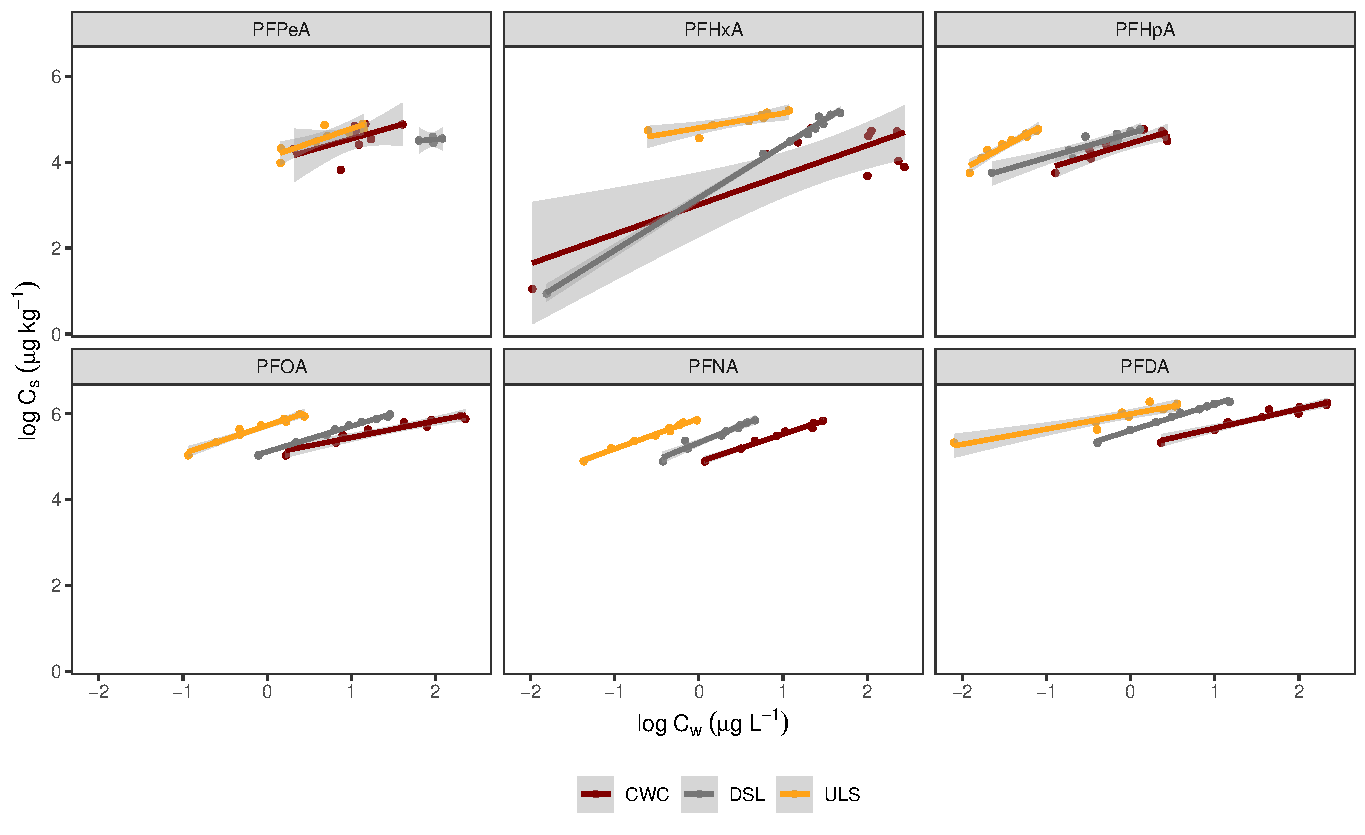
\includegraphics[width=\textwidth]{R/figs/Sorption_isotherms_single_BC.pdf}
    \caption{Sorption of PFCAs onto CWC biochar. Lines are the fitted Freundlich isotherms. Grey area represents the standard error.}
    \label{fig:Sorption_isotherms}
\end{figure}

\begin{figure}
    \centering
    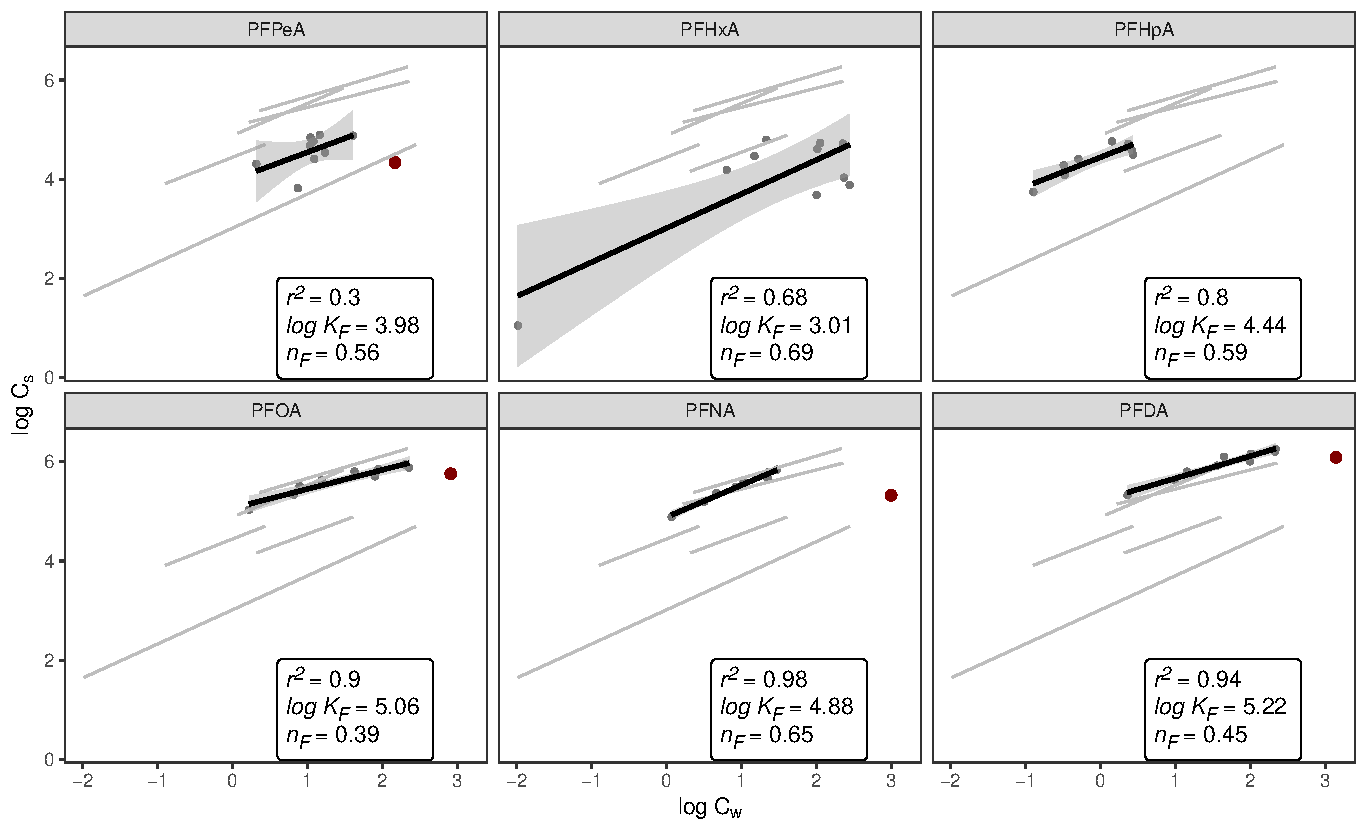
\includegraphics[width=\textwidth]{R/figs/CWC_facet_isotherm.pdf}
    \caption{Sorption of PFCAs onto CWC biochar. Lines are the fitted Freundlich isotherms.}
    \label{fig:CWC_isotherm}
\end{figure}

\begin{figure}
    \centering
    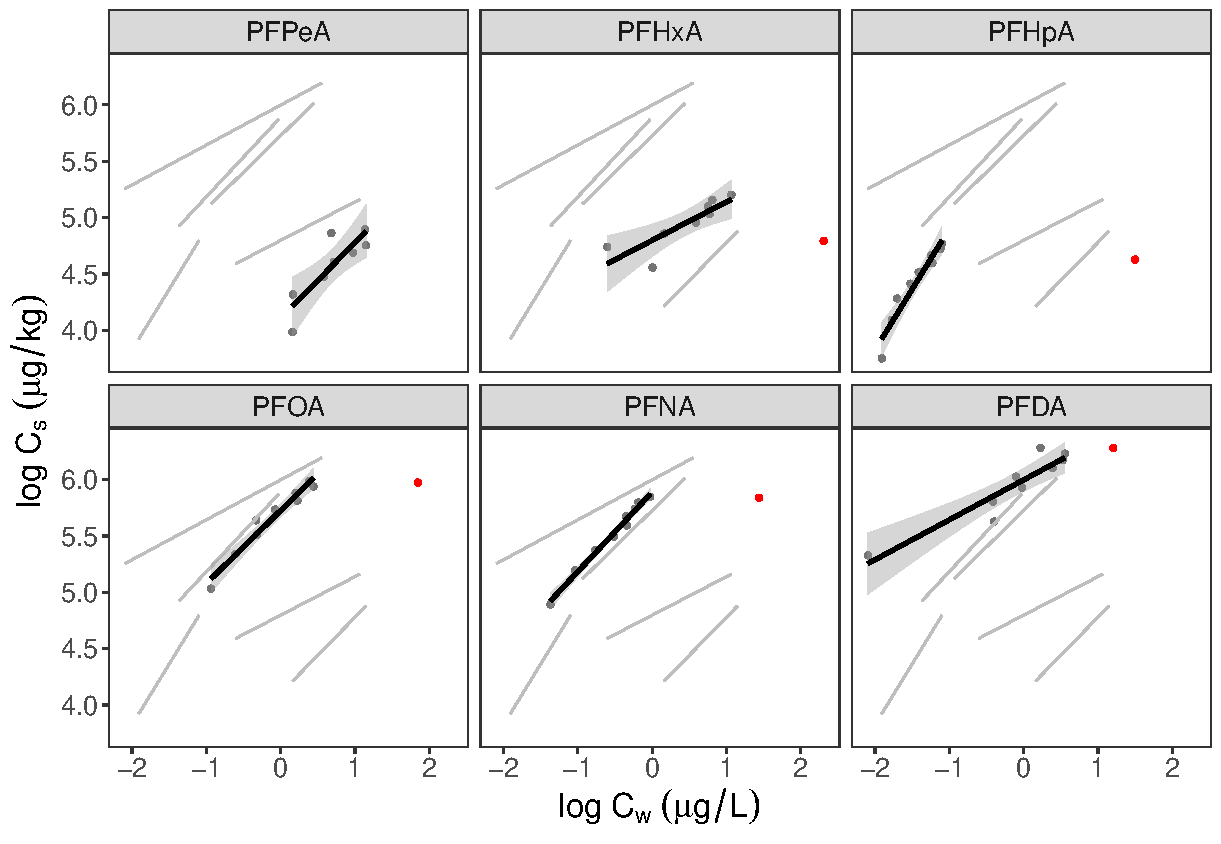
\includegraphics[width=\textwidth]{R/figs/ULS_facet_isotherm.pdf}
    \caption{ULS isotherm}
    \label{fig:ULS_isotherm}
\end{figure}

\begin{figure}
    \centering
    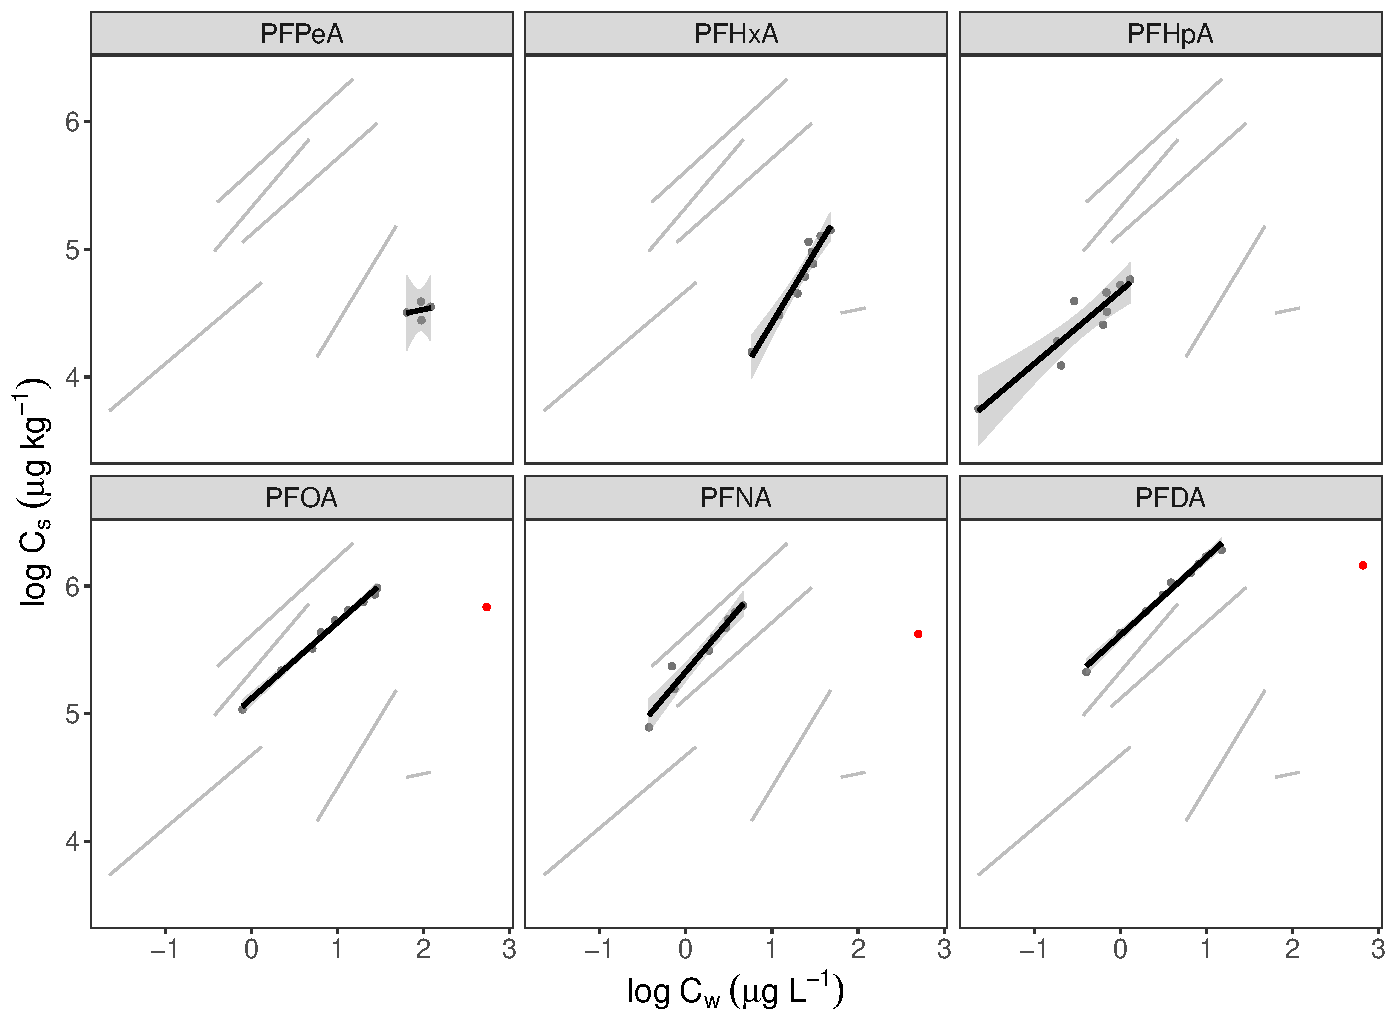
\includegraphics[width=\textwidth]{R/figs/DSL_facet_isotherm.pdf}
    \caption{DSL isotherm}
    \label{fig:DSL_isotherm}
\end{figure}

Table with partitioning coefficients for the biochar sorbents with and without the presence of soil, plus/minus standard error

\subsection{Freundlich parameters}

\begin{table}
\caption{Summary statistics for the single-compound 9-point isotherms for biochar-water. The error is presented as standard error.}
\centering
\adjustbox{max width=\textwidth}{%
\begin{threeparttable}
\label{tab:summary_stats_single}
\begin{tabular}{llllllllllll}
\toprule
\multicolumn{1}{c}{\textbf{Biochar}} & \multicolumn{1}{c}{\textbf{Compound}} & \multicolumn{3}{c}{\textbf{log K\textsubscript{F}}} & \multicolumn{3}{c}{\textbf{n\textsubscript{F}}} & \multicolumn{3}{c}{\textbf{r\textsuperscript{2}}} & \textbf{p} \\ \midrule
CWC                                  & PFPeA                                 & 3.98        & ±        & 0.36        & 0.56      & ±      & 0.33      & 0.30       & ±       & 0.31            & -             \\
CWC                                  & PFHxA                     & 3.01        & ±        & 0.32        & 0.69      & ±      & 0.17      & 0.68       & ±       & 0.67               & **           \\
CWC                                  & PFHpA                     & 4.44        & ±        & 0.05        & 0.59      & ±      & 0.11      & 0.80       & ±       & 0.16               & **           \\
CWC                                  & PFOA                      & 5.06        & ±        & 0.08        & 0.39      & ±      & 0.05      & 0.90       & ±       & 0.10               & ***          \\
CWC                                  & PFNA                      & 4.88        & ±        & 0.04        & 0.65      & ±      & 0.04      & 0.98       & ±       & 0.05               & ***          \\
CWC                                  & PFDA                      & 5.22        & ±        & 0.07        & 0.45      & ±      & 0.04      & 0.94       & ±       & 0.08               & ***          \\
DSL                                  & PFPeA                     & 4.25        & ±        & 0.74        & 0.14      & ±      & 0.38      & 0.06       & ±       & 0.07               & -             \\
DSL                                  & PFHxA                     & 3.16        & ±        & 0.04        & 1.22      & ±      & 0.03      & 1.00       & ±       & 0.09               & ***          \\
DSL                                  & PFHpA                     & 4.67        & ±        & 0.06        & 0.57      & ±      & 0.09      & 0.86       & ±       & 0.13               & ***          \\
DSL                                  & PFOA                      & 5.12        & ±        & 0.02        & 0.60      & ±      & 0.02      & 0.99       & ±       & 0.03               & ***          \\
DSL                                  & PFNA                      & 5.33        & ±        & 0.03        & 0.80      & ±      & 0.07      & 0.94       & ±       & 0.08               & ***          \\
DSL                                  & PFDA                      & 5.61        & ±        & 0.02        & 0.61      & ±      & 0.02      & 0.99       & ±       & 0.03               & ***          \\
ULS                                  & PFPeA                     & 4.10        & ±        & 0.13        & 0.67      & ±      & 0.16      & 0.74       & ±       & 0.17               & **           \\
ULS                                  & PFHxA                     & 4.80        & ±        & 0.06        & 0.34      & ±      & 0.09      & 0.72       & ±       & 0.13               & **           \\
ULS                                  & PFHpA                     & 5.98        & ±        & 0.17        & 1.08      & ±      & 0.11      & 0.93       & ±       & 0.10               & ***          \\
ULS                                  & PFOA                      & 5.73        & ±        & 0.02        & 0.65      & ±      & 0.05      & 0.95       & ±       & 0.07               & ***          \\
ULS                                  & PFNA                      & 5.89        & ±        & 0.02        & 0.71      & ±      & 0.03      & 0.99       & ±       & 0.04               & ***          \\
ULS                                  & PFDA                      & 6.00        & ±        & 0.04        & 0.35      & ±      & 0.05      & 0.86       & ±       & 0.13               & ***     \\ \bottomrule    
\end{tabular}
\begin{tablenotes}
\item Significant codes: *** $\sim$ 0.001, ** $\sim$ 0.01, - $>$ 0.05 
\end{tablenotes}
\end{threeparttable}}
\end{table}


Meaning of parameters KF and n
Importance of nonlinearity and concentration interval achieved 
Comparison of KF across concentration magnitudes, conversion factor and why

\subsection{Biochar sorbent properties vs sorption}
Carbon content of the biochars follows the expected trend, CWC \textgreater ULS \textgreater DSL with 91.4\%, 29.6\% and 13.5\%, respectively (\cref{tab:SAPV}). Oxygen content was highest for DSL and ULS (61.4 and 57.1 \% respectively) compared to 5.5 \% for CWC. CWC has a high C/O and C/H ratio (\textgreater 1) whereas ULS and DSL have ratios \textless 1. A high C/H and C/O ratio is associated with a high degree of aromaticity/condensation and few functional groups. This shows that the CWC matrix is dominated by carbon whereas ULS and DSL are dominated by oxygen resulting in a highly hydrophobic surface. The proportion of elements other than C, O, H and N contained in the biochar matrices is significantly different lower for the clean wood biochar (1.4 \%) compared to the sludge biochars (10.9 and 23.2 \%), containing a greater mixture of other elements. Total elemental composition of the three biochars is given in \cref{appSec:elements}.

Correlation plots:
    Iron speciation vs KF
    Surface area vs KF 
    Pore volume vs KF 
    C:O vs KF 
    C:H vs KF  
Discussion on how these factors influence sorption, sorption capacity and sorption affinity of biochars

\subsection{Influence of PFAS chain length}
For the three biochars conducted single-compound isotherms on, log K\textsubscript{d} increases linearly with fluorocarbon (CF) chain length (\cref{fig:chainlength}). Although the regression was not significant for CWC ($R^2$ = 0.64, p = 0.056), comparing the regression analyses all together is sufficient to confirm this relationship for all three biochars (can I say that?). For every CF\textsubscript{2} moiety, hydrophobic interactions between condensed aromatic structures in the biochar matrix increases. This suggests that hydrophobic interactions is the dominant sorption mechanism over electrostatic interactions between the anionic carboxylate functional group and positively charged surfaces on the sorbent. In accordance with most previous studies \citep{Sorengard2019,higgins2006sorption}. 

\begin{figure}
    \centering
    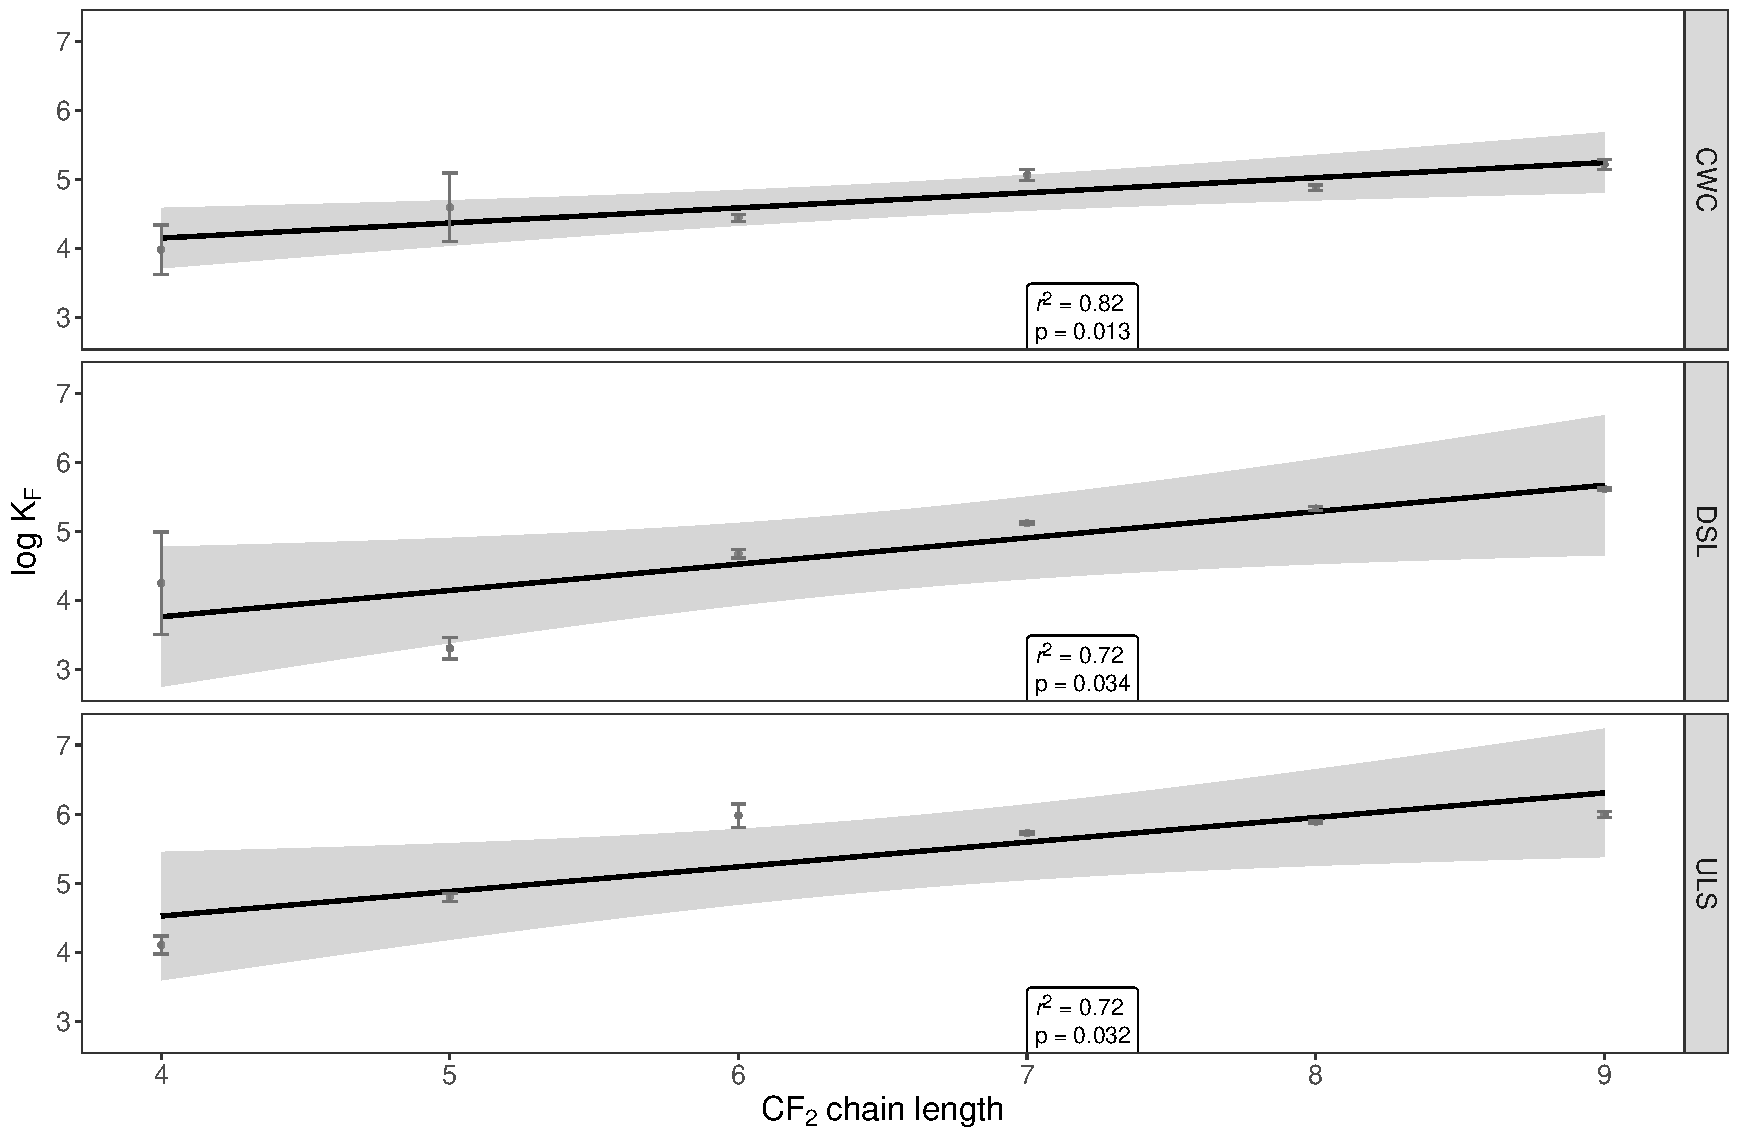
\includegraphics[width=\textwidth]{R/figs/chainlength_KF.pdf}
    \caption{Correlation plot of $log~K_F$ as a function of PFCA chain length (number of $CF_2$ moieties) for the different biochars fitted by a linear model. The error bars represent the standard deviation of $log~ K_F$ (n=9).}
    \label{fig:chainlength}
\end{figure}
 
Discuss reasons based on correlation plots
    hydrophobic effect, congeners comparison
    (find molecular size?)
    Biochar properties
        C/H, C/O ratio, 
        Porosity, surface area

\subsubsection{Influence of PFAS functional group}
Biochar properties
    Point of zero charge
    Surface functional groups, charge
    Iron content, charge
    Electrostatic interaction

\section{Biochar PFAS sorption efficiency: cocktail isotherms BC-water}
Biochar removal efficiency 
Freundlich parameters
Attenuation factors, larger for short-chain than long chains which have greater sorption affinity. 

\subsection{Competition}
Due to different spike concentration used for each compound in the cocktail, establishing quantitative trends for how chain length influences competition for sorption size is difficult. However, some conclusions can be drawn by looking at the overall trends. \cref{tab:competition} shows that $log~K_d$ decreases for all compounds in the presence of a mixture. $K_d$ changes the least for PFHxA and PFHpA (2.3 and 0.2 \% respectively) and may be attributed to lower spiked concentrations (330 and 117 \textmu g L\textsuperscript{-1}) for these compounds compared to the rest in \cref{tab:competition}. Competition is most profound for PFOA to CWC followed by PFDA for ULS and CWC (15.8, 10.0 and 10.6 \% respectively), which can be explained by the highest concentrations spiked for these compounds (1 953 and 3 830 \textmu g L\textsuperscript{-1}). It appears that sorption of PFNA is minimally influenced by competition between other compounds despite SC being in the higher range (1 409 \textmu g L\textsuperscript{-1}). $K_d$ for PFPeA is reduced by 8.2\% and is expected based on weaker sorption of short-chain compounds.

\begin{figure}
    \centering
    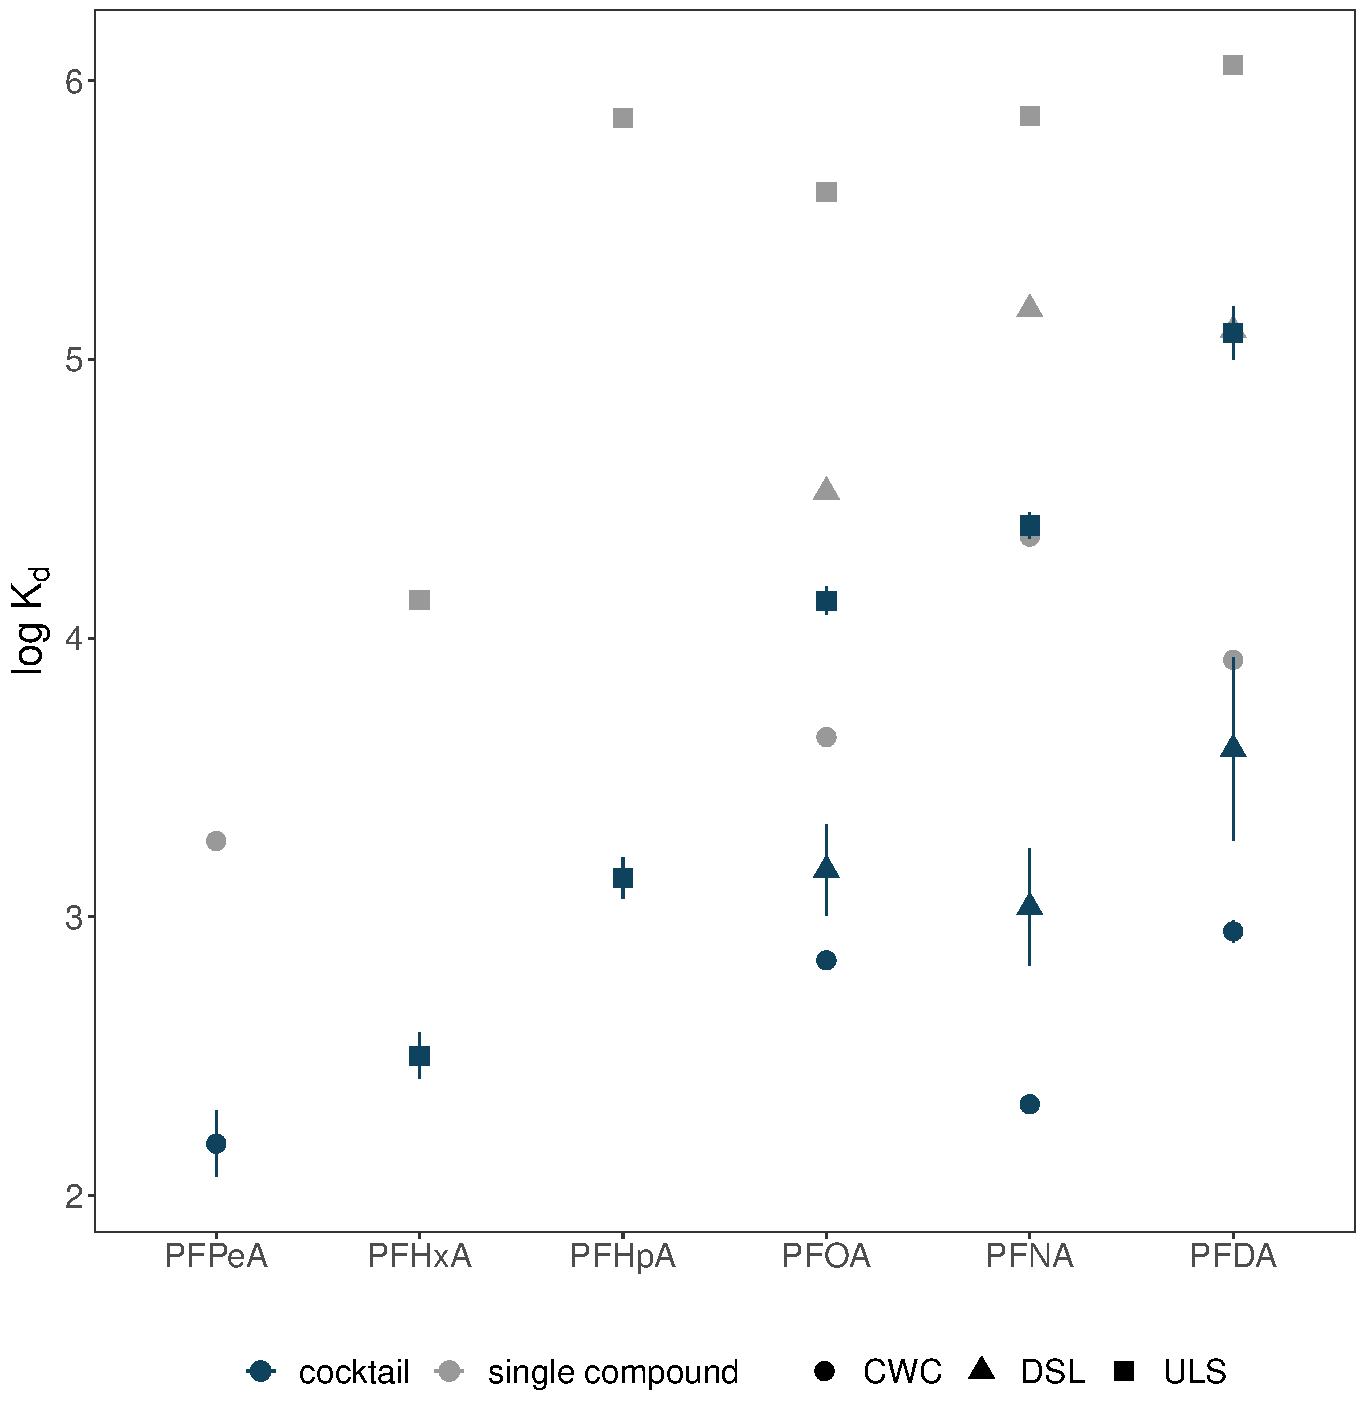
\includegraphics[width=\textwidth]{R/figs/C10_mixVsSingle_BC_plot.pdf}
    \caption{Sorption attenuation for TCs in a cocktail spiked at SC10. Note that the attenuation for cannot be compared across chain lengths as different concentrations have been used. The error bars represent the standard deviation of $log~K_F$ for the cocktail batch tests performed in triplicate. The single-compound $log~K_d$s are one point only.}
    \label{fig:competition}
\end{figure}

\begin{table}
\centering
\caption{Competition factor at SC10 (\cref{tab:spikeConcentrations}) for each compound and biochar. Competition factor is defined as K\textsubscript{d,single}/K\textsubscript{d,mix})$\times$100\%. For the compounds and biochars with blank cells (-), competition factors could not be calculated due to incomplete results.}
\label{tab:competition}
\begin{tabular}{lrrr}
\toprule
 & \multicolumn{3}{c}{Competition factor \%} \\ \cmidrule(l){2-4}
 & CWC & ULS & DSL \\ \midrule
PFPeA & 8.2 & - & - \\
PFHxA & - & 2.3 & - \\
PFHpA & - & 0.2 & - \\
PFOA & 15.8 & 3.4 & 4.4 \\
PFNA & 0.9 & 3.4 & 0.7 \\
PFDA & 10.6 & 10.9 & 3.1 \\ \bottomrule
\end{tabular}
\end{table}

\subsection{Surface area and pore volume}
Biochar from clean wood chips had a specific surface area (SSA) of 323  m\textsuperscript{2} g\textsuperscript{-1} for large pores (\textgreater 1.5 nm, N\textsubscript{2}), $\sim$ 200 m\textsuperscript{2} g\textsuperscript{-1} higher than the ULS and DSL sludge chars (128 and 110  m\textsuperscript{2} g\textsuperscript{-1}, respectively) \cref{tab:SAPV}. SSA of small pores (0.4-1.5 nm, CO\textsubscript{2} sorption) was 600  m\textsuperscript{2} g\textsuperscript{-1} for CWC, $\sim$ six times higher than ULS and DSL (165 and 87  m\textsuperscript{2} g\textsuperscript{-1}, respectively). Pore volume for large and small pores were relatively similar across biochar types (within 0.1 and 0.15 cm\textsuperscript{3} g\textsuperscript{-1} respectively). Contrary to previous findings, surface area and pore volume does not correlate with higher sorption as CWC proved to be the weakest sorbent in this study. A lack of significant linear correlations between SSA and $K_d$ and PV and K\textsubscript{d} is not surprising due to few biochar samples (n=3). 

Pore size distribution is important for explaining sorption of PFAS of increasing chain lengths due to differences in molecular size. PFDA has a maximum diameter of 1.54 nm, and therefore experiences size exclusion for the small pores (0.5-1.5 nm) and can therefore only diffuse into the larger pores represented by N\textsubscript{2} (\textgreater 1.5 nm) (\cref{tab:molecsize}). Regardless of the critical separation at pore size greater/less than 1.5 nm, shorter chain PFCAs is expected to diffuse more easily into the pores than the larger compounds.  

\begin{table}
\centering
\caption{Surface area, pore volume and elemental content (C, O, H, N) and ratios for the biochars produced for the batch tests.}
\adjustbox{max width=\textwidth}{
\label{tab:SAPV}
\begin{tabular}{lllllllllllll}
\toprule
Biochar & Pyrolysis   & \multicolumn{2}{l}{N\textsubscript{2} sorption}      & \multicolumn{2}{l}{CO\textsubscript{2} sorption}       & \multicolumn{4}{c}{Elemental content} & \multicolumn{3}{c}{Elemental ratio} \\
sorbent   & temperature & \multicolumn{2}{l}{(pores \textgreater 1.5 nm)} & \multicolumn{2}{l}{(pores 0.4-1.5 nm)} &         &         &         &         &             &           &           \\ \cmidrule(l){3-4} \cmidrule(l){5-6} \cmidrule(l){7-10} \cmidrule(l){11-13}
                & (\textdegree C)        & Surface area       & Pore volume     & Surface area       & Pore volume       & C       & O       & H       & N       & C/O         & C/H       & C/N       \\
                &             & ($\mathrm{m^2~g^{-1}}$)           & (cm\textsuperscript{3} g\textsuperscript{-1})       & ($\mathrm{m^2~g^{-1}}$)           & (cm\textsuperscript{3} g\textsuperscript{-1})         & (\%)     & (\%)     & (\%)     & (\%)     &             &           &           \\ \midrule
CWC         & 700         & 323                & 0.017           & 683                & 0.186             & 91.4    & 5.50    & 1.01    & 0.69    & 16.6        & 91        & 133       \\
ULS         & 700         & 128                & 0.126           & 165                & 0.047             & 29.6    & 57.1    & 1.24    & 1.13    & 0.52        & 24        & 26        \\
DSL         & 700         & 110                & 0.111           & 87                 & 0.027             & 13.5    & 61.4    & 1.05    & 0.82    & 0.22        & 13        & 16       \\ \bottomrule
\end{tabular}}
\end{table}


\begin{table}
\caption{Effective cross-sectional diameter (D\textsubscript{eff}) and maximum diameter (D\textsubscript{max}) of TCs interpolated and extrapolated by linear regression from calculations performed by \citep{inoue2012size} on PFOA and other PFCAs with chain lengths 11-18.}
\centering
\begin{threeparttable}
\label{tab:molecsize}
\begin{tabular}{llll}
\toprule
Compound & Carbon & D\textsubscript{eff} & D\textsubscript{max} \\ 
& chain & (nm) & (nm) \\
& length & & \\ \midrule
PFPeA    & 5                                                              & 0.45                                                 & 0.96                                                 \\
PFHxA    & 6                                                              & 0.50                                                 & 1.08                                                 \\
PFHpA    & 7                                                              & 0.56                                                 & 1.19                                                 \\
PFOA\textsuperscript{*}     & 8                                                              & 0.61                                                 & 1.36                                                 \\
PFNA     & 9                                                              & 0.67                                                 & 1.42                                                 \\
PFDA     & 10                                                             & 0.72                                                 & 1.54  \\ \bottomrule                                    
\end{tabular}
\begin{tablenotes}
\item \textsubscript{*} Calculated value from \citep{inoue2012size}
\end{tablenotes}
\end{threeparttable}
\end{table}

\subsection{Iron and copper speciation}
Synchrotron

\subsection{Elemental composition}

\subsection{PZC}

\subsection{PFAS sorption in single-compound batch tests with soil}
\subsection{Soil chemistry}
The soil used in the batch tests was characterized as a fine sand (0.1 to 0.3 mm) with 1.3 \% TOC (pH 5.38 \textpm 0.02 , CEC 2.63 \textpm 0.06 meqv 100 g\textsuperscript{-1}). Total element concentrations and exchangeable ion concentrations are in \cref{appSec:elements}, \cref{apptab:soil}. The soil extraction showed no native target analytes present.  


\subsection{pH and conductivity}
pH varied little between all biochar-soil-water systems with an average pH of 7.18 \textpm 0.02. Conductivity was 39 \textpm 0.9 \textmu S cm\textsuperscript{-1}. Since the variance is low, pH and conductivity was not considered as factors that influence sorption of PFCAs. The conductivity of soil-water samples differed the most from the rest of the samples with a mean conductivity of 23 \textpm 0.05 \textmu S cm\textsuperscript{-1} versus a mean of 41 \textpm 0.9 \textmu S cm\textsuperscript{-1} for the biochar-water and biochar-soil-water samples. Complete pH and conductivity data is in \cref{appSec:misclab}. 

\begin{table}
\centering
\caption{Mean pH and conductivity (\textmu S cm\textsuperscript{-1}) measurements for the different batch test systems (n=3). The error bars represent the standard error. BC:S:H\textsubscript{2}O is the biochar:soil:water ratio.}
\label{tab:pHcond}
\begin{tabular}{lccccc}
\toprule
 & \multicolumn{2}{c}{\textbf{pH}} & \multicolumn{2}{c}{\textbf{Conductivity}} & \\ \cline{2-5}
 & mean & std. dev & mean & std. dev & BC:S:H\textsubscript{2}0\\ 
\midrule
ULS & 7.10 & 0.04 & 45.70 & 3.03 & 1:0:500\\
DSL & 7.31 & 0.02 & 40.93 & 1.07 & 1:0:500\\
CWC & 7.36 & 0.07 & 46.47 & 0.70 & 1:0:500\\
ULS+S & 7.18 & 0.02 & 34.93 & 0.40 & 1:50:500\\
DSL+S & 7.14 & 0.00 & 35.73 & 1.50 & 1:50:500\\
CWC+S & 7.09 & 0.05 & 44.90 & 1.54 & 1:50:500\\
S & 7.08 & 0.05 & 23.33 & 0.87 & 0:1:10\\
\bottomrule
\end{tabular}
\end{table}


\section{Biochar PFAS sorption efficiency: single-compound isotherms BC-soil-water}
Kd at C10 for soil alone
How to account for Kd of soil when calculating KF 
    Show how to derive Freundlich equation with respect to soil Kd from original Freundlich equation
    
\subsection{PFOA isotherms vs cocktail isotherms}
to compare with C$_w$ at SP10 for the single compound batch test to determine a competition factor between the other PFCAs in the cocktail to sorption sites on the biochar.

Plot comparing the isotherms of PFOA-BC to PFOA-soil-BC
Discuss influence of presence of soil on PFOA sorption
Significance of C8 chain length taken together with BC properties 

Plot comparing cocktail-BC to cocktail-soil-BC
Effect of presence of soil AND competing congeners
Competitive sorption, attenuation factor

Comparison between sorption of PFOA in cocktail-soil and PFOA in biochar-soil

\subsection{Sorption attenuation by soil}
fouling/pre-loading by NOM
Pore blocking

\subsection{Soil-BC interactions}
Most previous studies have reported a linear increasing trend between log Kd and chain length. However not for PFPeA, \citep{zhang2013sorption}, found in \citep{Sorengard2019}. and \citep{guelfo2013}  these studies are for sorption to organic matter.  Steric hinderance. 

\subsubsection{Difference in color of filtrate between batch tests}
Filter clogging and reduction in filter size, had to exchange filters during filtration, how this may impact results
Aggregation of humic substances upon addition of acetic acid pre-SPE, how this may impact results

Precipitation of a brown fluff was observed when filtered batch tests containing soil was adjusted to pH 3 with 1 M acetic acid

\begin{figure}
    \centering
    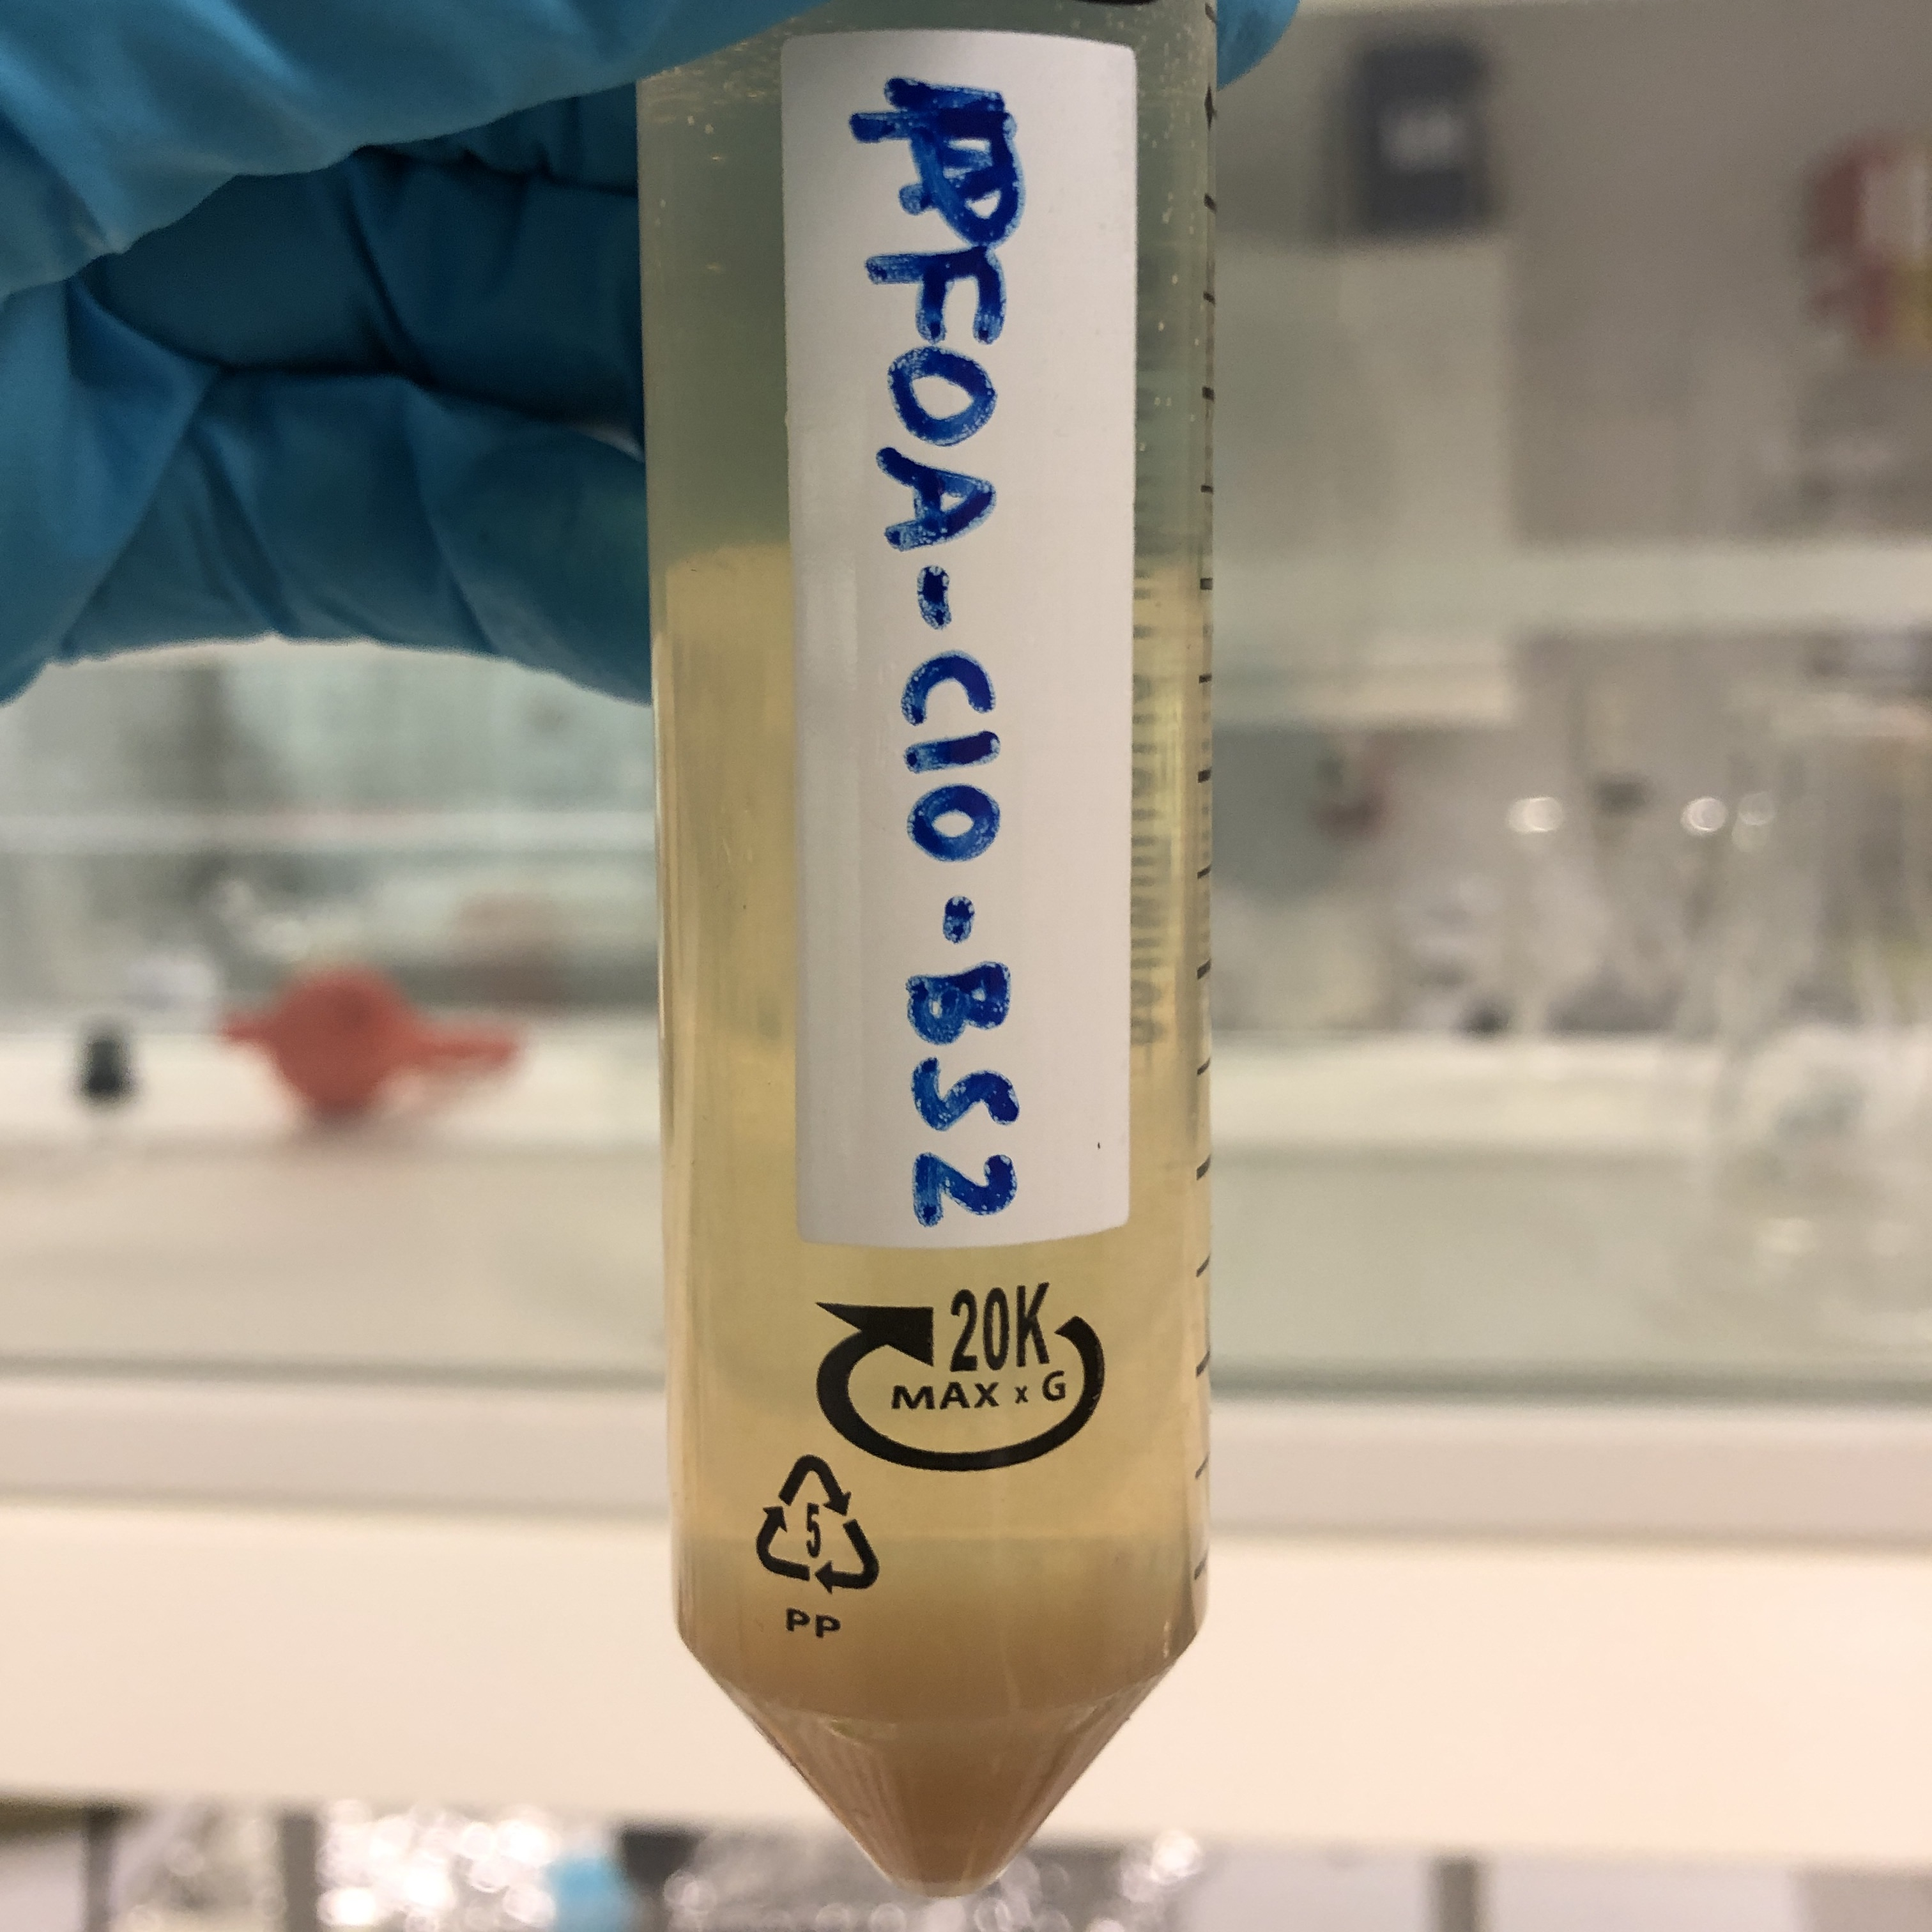
\includegraphics[width=0.6\linewidth,scale=0.6]{Bilder/Samples/Precipitation.jpg}
    \caption{Precipitation observed when filtered soil samples were adjusted to pH 3 with 1 M acetic acid.}
    \label{fig:precip}
\end{figure}

\section{Potential for commercializing sludge chars as sorbents}
\subsection{Sorbent quality}
Removal efficiency, good enough for application?
\subsubsection{EBC limits heavy metals}
Leaching of heavy metals results at PT 700 C
    As, Cd, Co, Zn, Pb for all chars Below EBC limits, Cr and Ni between lower and upper limit
    EBC = European Biochar Certificate
    Cu above EBC limits for ULS and DSL
    Enrichment factors heavy metals (?)

\subsubsection{Field conditions representativeness}
Soil pH, sorption/desorption of PFAS
Protonation state of PFAS (pKa) unaffected at environmentally relevant pH’s
Leaching in acid soil not a problem, will increase sorption affinity of charged carboxyl to protonated BC surface
Alkaline conditions, liming?? 
    Depends on the dominating sorption mechanism
    Repulsion: functional groups, iron oxides, changes charge with pH?
    If hydrophobic interactions are dominating, sorption will likely not be affected
Equilibrium conditions vs laboratory batch tests
BC dose

Are the results representative of what goes on in real life? Sorption by shaking for 14 days represent an assumed equilibrium between PFCAs in the water and soil phase. A comparable situation in the field would be washing of the soil with large amounts of water such as during heavy rainfall. This will only be the case during occasional stormwater events and thus the results from this research could benefit from being supplemented with results from leaching tests using biochar mixed with soil. However, the relationship:

\begin{align}
    \frac{k_1}{k_2}
\end{align}

where \(k_1\) is the PFCA sorption (adsorption and absorption) rate and \(k_2\) is the PFCA desorption rate, where \(k_1>>k_2\), which indicates that sorption is many times higher, and in an equilibrium situation, sorption and desorption will be at steady state \citep{Cornelissen2005}. 


\section{Sustainability}
\subsection{Pyrolysis energy demand}
\subsection{Life cycle impact assessment (LCIA)}
LCA (life cycle assessment), sustainability aspects of production of biochar
High operating energy and cost different technologies \citep{Alhashimi2017}

\section{Quality control of laboratory analysis and uncertainty}

\subsection{Spiking standard concentrations}
SPE and directly, why?

The pipettes used for making the PFCA dilutions were calibrated. The three pipettes were: 1) 2-10 mL, 2) 200-1000 \textmu L, and 3) 5-50 \textmu L. All pipettes were below the permitted coefficient of variation (CV = 0.3, 0.5, and 2 $\%$ respectively (\cref{appSec:misclab}, \crefrange{appTab:pip2-10}{appTab:pip5-50}).

Since the diameter of the centrifuge tube (30 mm) was larger than that of a volumetric flask and biochar was added prior to the dilution process, the final concentration of the sorbent-sorbate mixture may have a heightened inaccuracy. However, the volume of which 0.1 g biochar occupies can be considered insignificant due to the high absorptive capacity of biochar and small mass used. Therefore a set of 10 centrifuge tubes filled to 50 mL containing 0.1 g CWC were weighed to control the uncertainty of the final dilutions. The results from weighing show that the weight of 10 trials were not accurate but precise, which means that all samples were prepared with the same final volume even though this volume deviates from 50 mL (\cref{appTab:PPcentrifuge}). 

Volume 50 mL weighed vs by eye measurement, diameter of test tube and error
preparation of cocktail standard, not consistent, some individual pipetting. 

\subsubsection{Filter blanks no significant difference}

\subsection{PFAS losses during laboratory analysis}
SPE protocol, many steps, many PP test tubes transfers, saturated PFAS-solutions, internal standard (dilutions had to disregard IS because too low concentration)

\citep{Lath2019labsorb}: 
Syringe filters: sorption of PFOA to centrifuge tubes and filter membranes. Sorption onto syringe surface: negligible due to short residence time (\textless 10 s). 74\% recovery from regenerated cellulose syringe filter. No improvement in recovery was seen when conditioning the syringe filters with phosphate solution or methanol. No trend between losses of PFOA on syringe filter and increasing spike concentrations. Centrifugation only is therefore advised if possible to avoid filtration losses. 

Test tubes: Greater recoveries from glass tubes than plastic, PP poorest recovery (55-68 \% recovery)... Contact time of PFAS residing in tubes for longer than 7 days should not be of significance, as \citep{Lath2019labsorb} propose that sorption and saturation of tube walls occur within hours. 74-81 \% recovery for PP when testing dependence on pH and ionic strength. Slight pH dependence, higher recovery at higher pH due to repulsion of negatively charged functional groups (PP has negative surface charge above pH 3.5-4. Bridging effect will be observed at higher pH's between cations like Ca2+, but is still considered negligible compared to the losses due to the physicochemical properties of the materials themselves. In general PP and plastics consists of mainly carbon hydrogen chains and are more hydrophobic than glassware. Sorption to tube walls saturate, so recoveries increase significantly with higher spike concentrations (e.g. for PP, 12-415 ug/L spiked PFOA increased recovery from 53.7-85.5 \%). Therefore, quantification of low concentrations may be subject to highest error, and in most cases will be an underestimation of dissolved concentrations. 

Use of PP test tubes, study
Higher probability of underestimating Cw for low-concentration samples because tube walls saturate – maximum number of sorption sites, there is a sorption maximum (Langmuir)

\subsection{Uncertainty}
\subsubsection{Batch tests}
Vel, du kan jo prøve å legge sammen alle de feilene. Det finnes jo forskjellige typer feilkilder i et stort forsøksoppsett. Det man ofte ser er at det er en eller to feil som er så store at de overskygger de andre. Da er det ikke noen vits å ta med alle de små. Feilen som ofte er størst er reproduserbarhet av metoden. Altså forskjellen mellom for eksempel prøver laget i triplikater. Det du kan gjøre i oppgaven din er jo å kort diskutere feilkildene du har og identifisere de største og viktigste.

\subsubsection{Analytical}
Calibration curves and matrix effect
LC-MS/MS

\subsubsection{Peak integrations}
Manual review of peak integrations
decisions to remove C1 at low signal
where observed similar peak integrations across concentrations, suspected saturation of detector, dilution of these samples

\subsubsection{Mass balance filters/BC and water}
Why chose only to analyze aqueous phase


\section{Biochar analyses and characterization}

\subsection{Biochar properties}
Table of pyrolysis yield, ash content, caloric content etc. 

\subsection{Enrichment factor}
Calculation of enrichment factor for C – potential for carbon storage
mention ETIA measurements

\section{Biochar properties}

